\index{data set}
\index{nominal variables}
\index{multilayer perceptron}
\index{performance functional, pattern recognition}
\index{training algorithm, pattern recognition}
\index{underfitting}
\index{overfitting}
\index{regularization theory}
\index{early stopping}
\index{classification accuracy}
\index{error rate}
\index{sensitivity}
\index{specifity}
\index{confusion matrix}
\index{true positives}
\index{false positives}
\index{true negatives}
\index{false negatives}

\subsection*{Introduction}

Another traditional learning task for the neural networks is the pattern recognition (or classification) problem \cite{Bishop1995}. 
The task of pattern recognition can be stated as the process whereby a received pattern, characterized by a distinct set of features, 
is assigned to one of a prescribed number of classes. 
Here the neural network learns from
knowledge represented by a data set consisting of input-target examples.
The inputs include a set of features which characterize a pattern. The targets specify
the class that each pattern belongs to.

Therefore, in order to solve a pattern recognition problem, the input space must
be properly separated into regions, where each region is assigned to a class. A border
between two regions is called a decision boundary. The goal in a pattern recognition problem 
 is thus to obtain a neural network function as an
approximation of the pattern recognition function.


The formulation of a pattern recognition problem requires:

\begin{itemize}
\item[-] A data set. 
\item[-] A neural network.
\item[-] A performance functional.
\item[-] A training strategy.
\item[-] A model selection algorithm.
\item[-] A testing method.
\end{itemize}

A common feature of most data sets is that the data
exhibits an underlying systematic aspect, represented by some
function, but is corrupted with random noise. 

The central goal is to produce a model which exhibits good generalization, or in other words, one which makes good predictions for new data. The best generalization to new data is obtained when the mapping represents the underlying
systematic aspects of the data, rather capturing the specific
details (i.e. the noise contribution) of the particular data set. 

\subsection*{Data set}

In pattern recognition a pattern is represented by a set of attributes, viewed as a multi-dimensional feature vector. 
They are associated with one of a prescribed number of classes, which are in general of nominal nature.  

Table \ref{PatternRecognitionDataSetTable} shows the format of a data set for pattern recognition.
It consists of $n$ input variables and $m$ target variables,
comprising $q$ instances.

\begin{table}[h!]
\begin{center}
\begin{tabular}{|ccc|c|}
\hline
$input_{1,1}$ & $\ldots$ & $input_{1,n}$ & $\mathcal{class}_{1}$\\
$input_{2,1}$ & $\ldots$ & $input_{2,n}$ & $\mathcal{class}_{2}$\\
$\vdots$  & $\vdots$ & $\vdots$  & $\vdots$\\ 
$input_{q,1}$ & $\ldots$ & $inputx_{q,n}$ & $\mathcal{class}_{q}$\\
\hline
\end{tabular}\caption{Data set for pattern recognition.}
\label{PatternRecognitionDataSetTable}
\end{center}
\end{table}

As we have said, the target variables are nominal variables,
Therefore, for numerical computation, they need to be given numerical values. 

For the case of two classes, the number of target variables will be just one.
One class can be simply codified as $0$ and the other as $1$. 
For instance, in a medical diagnostic application, we can assign the value $0$ to a sane person and $1$ to an ill person.

For the case of multiple classes  the target data can be codified with a $1$-of-$m$ scheme. 
For instance, consider a food industry which needs to classifying fishes into $3$ species. 
That species can be given the targets $(1,0,0)$, $(0,1,0)$ and $(0,0,1)$, respectively. 

Note that some attributes can also be of nominal nature. 
In this case the same coding scheme as that described above for the targets will be used for the inputs. 

A simple statistical analysis must be always performed in order to check
for data consistency. Basic statistics of a data set for pattern recognition include the
mean, standard deviation, minimum and maximum values of the input variables and the frequency of the different classes. 

Also, it is a must to scale the input data. 
Either the mean and standard deviation or the and the minimum and maximum methods can be used for this purpose. 
Note that the target data has already proper $0$ and $1$ values. 

It is also convenient to split the data set into a training, a generalization and a testing subsets.
The size of each subset is up to the designer, but ratios of $60\%$, $20\%$ and $20\%$ are quite common. 
The data can be divided at random or by specifying given indices. 

The neural network represents the pattern recognition function. 
The number of inputs must be equal to the number 
of inputs in the data set, and the number of outputs must be the number of targets. 
The basis of this neural network is a multilayer perceptron. 
It might also include a scaling layer for the inputs, and a probabilistic layer for the outputs. 
On the other hand, the complexity of the neural network is up to the designer. 
This complexity will be given by the number and the sizes of the layers in the multilayer perceptron. 
Figure \ref{NeuralNetworkPatternRecognitionFigure} shows a neural network to be used for pattern recognition. 

\begin{figure}[h!]
\begin{center}
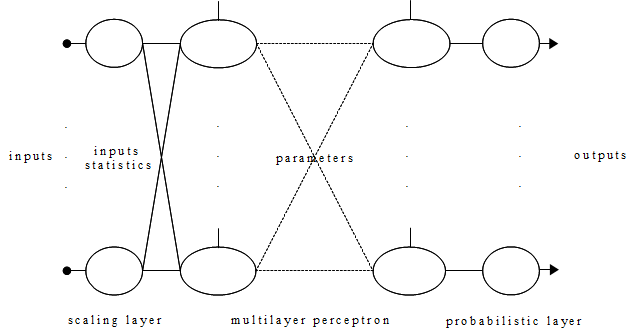
\includegraphics[width=1.2\textwidth]{pattern_recognition/neural_network_pattern_recognition.png}
\caption{Neural network for pattern recognition.}\label{NeuralNetworkPatternRecognitionFigure}
\end{center}
\end{figure}

In general, a multilayer perceptron with two layers is enough. 
A common activation function for the first layer is a sigmoid, such as the hyperbolic tangent or the logistic. 
Let us consider the activation function which should be used for the output layer. 

If the number of classes is two, the number of outputs in the neural network will be one. 
Therefore, a logistic activation function will interpret the outputs as probabilities, since it lies in the range $(0,1)$,
and no probabilistic layer is needed here. 

For multiple classes, we can use a multilayer perceptron with linear output layer. 
A probabilistic layer with softmax method is then added to form the neural network in Figure \ref{NeuralNetworkPatternRecognitionFigure}.

\subsection*{Performance functional}

In pattern recognition problems, the performance functional evaluates quantitatively the performance of the pattern recognition function against the data set. 
It is of the form

\begin{eqnarray}\label{PerformanceFunctionalPatternRecognition}\nonumber
\text{performance functional}=\text{objective term}+\text{regularization term}.
\end{eqnarray}

Common objective functionals for function regression, such as the sum squared error, the mean squared error, the root mean squared error, the normalized squared error and the Minkowski error are also commonly applied for pattern recognition. 
However, there are specific problems for this learning task, such as the cross-entropy error.

\subsection*{Training strategy}

The training algorithm for pattern recognition problems applies in the same way as for function regression problems. 

\subsection*{Model selection}

The problems of underfitting and overfitting also might occur when solving a pattern recognition problem with a neural network. 
Underfitting is explained in terms of a too simple decision boundary which gives poor separation of the training data. 
On the other hand, overfitting is explained in terms of a too complex decision boundary which achieves good separation of the training
data, but exhibits poor generalization.

A method for preventing underfitting and overfitting is to use a network that is just large enough to provide an adequate fit. 
An alternative approach to obtain good generalization is by using regularization theory.

As in function regression, early stopping can also be performed in pattern recognition to prevent overfitting. 
However, this technique usually produces underfitting and a more precise model selection analysis is preferible. 

\subsection*{Testing analysis}


The classification accuracy, error rate, sensitivity, specifity positive likelihood and negative likelihood are parameters for testing the performance of a pattern recognition problem with two classes. 

The classification accuracy is the ratio of instances correctly classified,  

\begin{eqnarray}\nonumber
\text{classification accuracy} = \frac{\text{true positives} + \text{true negatives}}{\text{true positives}+\text{true negatives}+\text{false positives}+\text{false negatives}}.
\end{eqnarray}

The error rate is the ratio of instances misclassified, 

\begin{eqnarray}\nonumber
\text{error rate} = \frac{\text{false positives} + \text{false negatives}}{\text{true positives}+\text{true negatives}+\text{false positives}+\text{false negatives}}.
\end{eqnarray}

The sensitivity, or true positive rate, is the proportion of alcual positive which are predicted positive, 

\begin{eqnarray}\nonumber
\text{sensitivity} = \frac{\text{true positives}}{\text{true positives}+\text{false positives}}.
\end{eqnarray}


The specifity, or true negative rate, is the proportion of actual negative which are predicted negative, 

\begin{eqnarray}\nonumber
\text{specifity} = \frac{\text{true negatives}}{\text{true negatives}+\text{false positives}}.
\end{eqnarray}
 
The positive likelihood is the likelihood that a predicted positive is an actual positive

\begin{eqnarray}\nonumber\label{PositiveLikelihood}
\text{positive likelihood} = \frac{sensitivity}{1-specifity}.
\end{eqnarray}

The negative likelihood is the likelihood that a predicted negative is an actual negative

\begin{eqnarray}\nonumber
\text{negative likelihood}= \frac{specifity}{1-sensitivity}.
\end{eqnarray}

Table \ref{BinaryClassificationPerformanceVariables} summarizes the binary classification performance variables

\begin{table}[h!]
\begin{center}
\begin{tabular}{c}
\hline
Classification accuracy\\
Error rate\\
Sensitivity\\
Specifity\\
True positive rate\\
True negative rate\\
\hline
\end{tabular}\caption{Binary classification performance variables.}
\label{BinaryClassificationPerformanceVariables}
\end{center}
\end{table}


In the confusion matrix the rows represent the target classes and the columns the output classes for a testing target data set. The diagonal cells in each table show the number of cases that were correctly
classified, and the off-diagonal cells show the misclassified cases. 

For the case of two classes the confusion matrix takes the form

\begin{eqnarray}\nonumber
\mathbf{C} = 
\left(
\begin{array}{cc}
\text{true positives} & \text{false positives} \\
\text{false negatives} & \text{true negatives} \\
\end{array}
\right).
\end{eqnarray}

% ROC CURVES

